\section{Half-Edge-Mesh}
Um die oben genannten Problemstellungen zu l\"osen, gibt es andere Ans\"atze Polygonalnetze zu realisieren. Einer dieser L\"osungen ist das Konzept der Half-Edge-Meshes. Ein solches Mesh besteht aus folgenden Komponenten: 
\begin{itemize}
	\item eine Liste von Vertices
	\item eine Liste von Half-Edges
	\item eine Liste von Faces.
\end{itemize}
Der Ansatz des Half-Edge-Mesh sieht dabei vor, dass jede Kante des Netzes aus zwei Half-Edges besteht, sodass jeweils eine Half-Edge auf einen Vertex der Kante zeigt, wie in Abbildung \ref{fig:half-edge-mesh} gezeigt.
Jede Half-Edge besitzt eine Referenz auf die ihr gegen\"uberliegende Half-Edge und auf die ihr Nachfolgende. Zudem referenziert sie die anliegende Face und den Vertex, aus dem sie hervorgeht.
\begin{figure}[t]
	\centering
	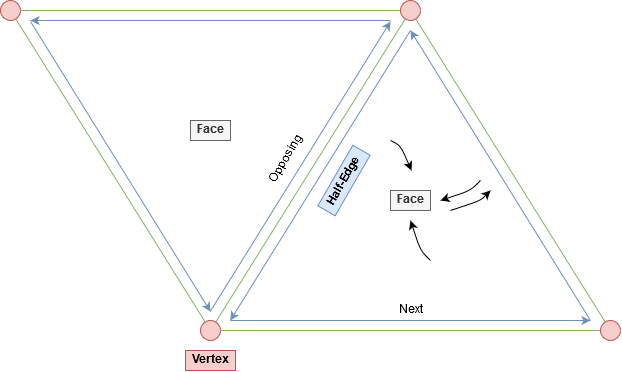
\includegraphics[width=0.7\linewidth]{Images/half-edge-mesh}
	\caption[Half-Edge-Mesh Schematik]{Die Elemente eines Half-Edge-Mesh.}
	\label{fig:half-edge-mesh}
\end{figure}


